\chapter{Installation}
\label{ch:Installation}

To run a Drupal website, 3 things are needed:
\begin{itemize}
    \item A WebServer, i.e. Apache
    \item A Database, i.e. MariaDB, MySQL, SQLite...
    \item A PHP Runtime Environment
    
\end{itemize}


These requirements can be hosted online via AWS, Combell, Pantheon.io... or you can set up a local development environment via an AMP stack. Depending on your operating system, there are multiple options. On Windows, XAMPP can provide this development environment, but you can also use Docker to containerize and set up a Lando Development Environment.

Whatever environment you choose, it is always recommended to manage your Drupal website via composer. In the following sections, we'll setup a XAMPP environment and install all necessary tools to get started. We'll also reference some options.

\section{XAMPP}
\label{sc:xampp}
When we want to download XAMPP\footnote{https://www.apachefriends.org/download.html}, there are different versions, linked to the PHP version that is included. Depending on the Drupal Version you want to install, you need to have PHP version support. Always check the release notes or official documentation to know the right Drupal version requirement. Drupal version 10.1 needs PHP version 8.1 or higher\footnote{https://www.drupal.org/docs/getting-started/system-requirements/php-requirements}.

On the moment of writing, PHP version 8.2.4 is the latest version supported by XAMPP, so that would be the best choice to be future-proof as well. If you want to host an older version of Drupal or have a legacy site to maintain, be sure to have the right environment.

Once XAMPP is installed, run the application and make sure Apache and MySQL are up and running.

\begin{figure}[h]
    \centering
    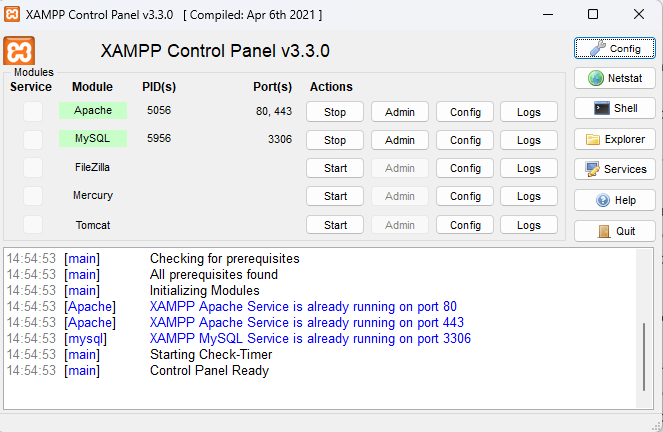
\includegraphics[width=1\linewidth]{img/ch2/xampp}
    \caption{XAMPP Control Center}
    \label{fig:xampp}
\end{figure}

To make sure we can install Drupal and run it smoothly, we need to change some configuration for Apache and MySQL. This can be done using the Config buttons in the XAMPP Control Panel for each service.

First we need to enable the PHP Extension GD. Go to the PHP.ini file via the Apache Config and remove the semi-colon that comments out the extension gd.

\begin{minted}{bash}
    extension=gd
\end{minted}

Be sure to re-start Apache once the settings have been changed.

\section{Composer}
Composer is an application-level package manager for the PHP programming language that provides a standard format for managing dependencies of PHP software and required libraries. 
It is the most recommended tool to install Drupal.
It will be used during the course to install, extend and manage Drupal.

Composer can be installed on all operation systems, it only needs a PHP installation.
In our case we've installed PHP by installing XAMPP in \ref{sc:xampp}.

    Detailed instructions to download and install composer can be found on the official website\footnote{https://getcomposer.org/download/}


\section{Other options}
As mentioned before, there are a number of other options that can be used to host Drupal Websites. Below we'll highlight a few which might be useful to look at.
\subsection{Pantheon.io}
Taken from the Pantheon website\footnote{https://pantheon.io/}:

\begin{quote}
Pantheon is the single SaaS platform provider that affordably integrates website development, management, performance, team education and hands-on account support. All with enterprise-grade security and the world's fastest hosting. All in one secure environment.
\end{quote}

Especially when working with a team, it can be interesting to host your Drupal website on Pantheon. You can all share the same development environment and the code is stored in a GIT repository which can be cloned and ran locally as well.

Open a free account and create a new Drupal 10 website with an easy wizard.

\subsection{Combell}
Combell is a webhosting company where you can host your own website and provides domainname registration as well.

Via AcademicSoftware\footnote{https://www.academicsoftware.eu/}, a student of Hogeschool Gent can request free hosting, which also includes a domainname. 

Several packages are possible, but for Drupal make sure to take the Combell Web Hosting (Linux) package. 

Once acquired, you can create up to 4 websites on that hosting. You can access the hosting via SFTP or SSH, or use the one-click install to launch a CMS like Drupal, Wordpress or Joomla.


\subsection{Docker Lando}
As a final noteworthy mention, there is Lando\footnote{https://lando.dev/}. A one-stop shop for creating a dev environment. Lando uses a Docker engine backend and can run on Windows, MacOS and Linux.

For Windows the WSL2 feature needs to be enables. You can find all the details on the documentation website\footnote{https://docs.lando.dev/getting-started/installation.html}.




